\section{Kubernetes}

In this section we will dive into the topic of Kubernetes. We start by shortly overviewing the Kubernetes architecure. Then we expand on the Kubernetes resources, their kinds and their role in the target application environment. Finally, we consider some of the security aspects of the Kubernetes and its varieties.

\subsection{Overview}

Kubernetes, also known as K8s, is an open source system for automating deployment, scaling, and management of containerized applications. It groups containers that make up an application into logical units for easy management and discovery. Kubernetes builds upon 15 years of experience of running production workloads at Google, combined with best-of-breed ideas and practices from the community \cite{kubernetes}.

IBM defines Kubernetes as an open source \textbf{container orchestration platform} for scheduling and automating the deployment, management and scaling of containerized applications. Today, Kubernetes and the broader ecosystem of container-related technologies have merged to form the building blocks of modern cloud infrastructure. This ecosystem enables organizations to deliver a highly productive hybrid multicloud computing environment to perform complex tasks surrounding infrastructure and operations. It also supports cloud-native development by enabling a build-once-and-deploy-anywhere approach to building applications \cite{ibm-kubernetes}.

It is important to emphasize that the Kubernetes abstracts the actual machines (nodes) from the user. Nodes can be physical on-premises servers, or VMs that reside either on-premises or at a cloud provider. Kubernetes takes on the responsibilty of figuring out the deployment target for a particular application. That is, user only defines the desired state of the infrastructure using YAML or JSON configuration files. Kubernetes then creates all the workloads based on the applied configuration.

\subsection{Kubernetes Architecture}

While Kubernetes requires at least three nodes to run, there are some implementation designed for the local use, which emulate this concept (see Subsection~\ref{sec:other-kubernetes-implementations}). The master node is called control plane. The control plane manages the worker nodes and the Pods in the cluster. In production environments, the control plane usually runs across multiple computers and the cluster runs multiple nodes, providing fault-tolerance and high availability. Worker nodes host the actual workload inside the cluster. Figure~\ref{img:kubernetes-architecture} provides a simple high-level overview of a typical Kubernetes cluster with a Control Plane and three worker nodes.

\begin{figure}[!hbt]
	\begin{center}
		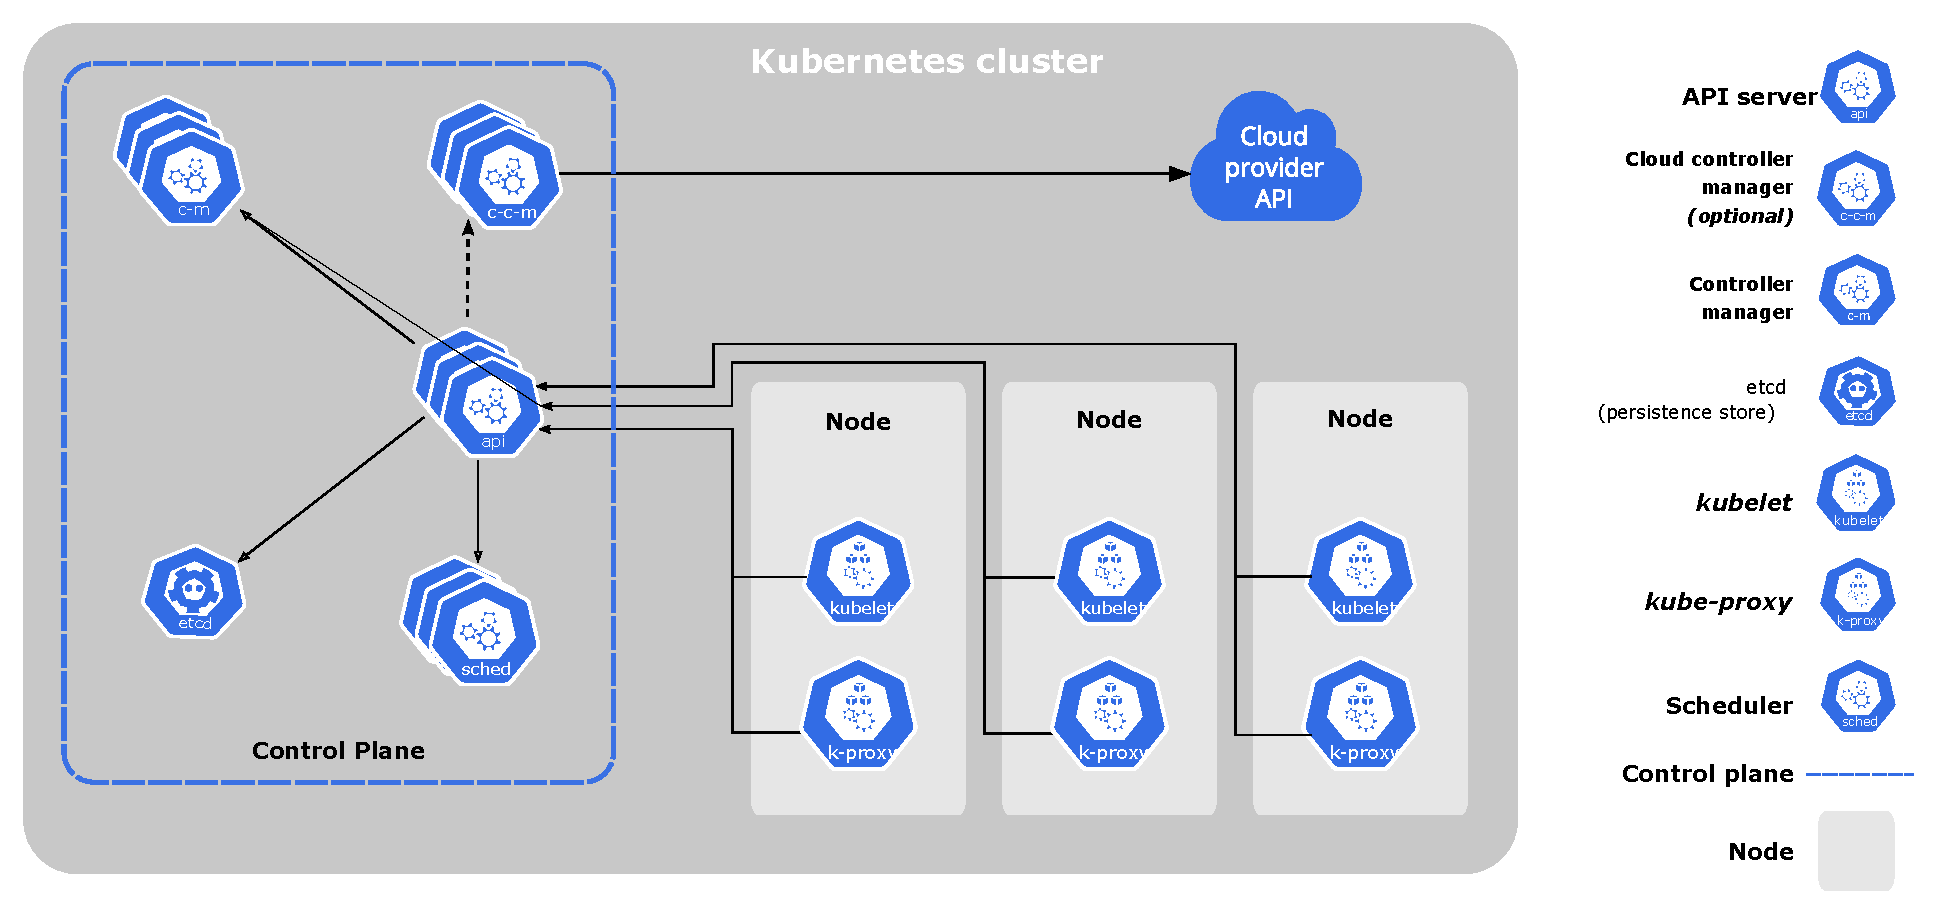
\includegraphics[width=0.85\textwidth]{images/components-of-kubernetes.pdf}
        \caption{Kubernetes cluster architecure overview with its main components \cite{kubernetes-components}.}
		\label{img:kubernetes-architecture}
	\end{center}
\end{figure}

\subsubsection*{Control Plane overview}

Control plane runs the following components: 
\begin{itemize}
\item \textbf{kube-apiserver} \\
Kube-apiserver exposes the Kubernetes API, which is acting as a frontend for the Kubernetes control plane.
\item \textbf{etcd} \\
Etcd is a key-value store, where all of the cluster data is stored.
\item \textbf{kube-scheduler} \\
Each time a new pod is created, it is passed to the kube-scheduler, which assigns the pod to the specific node to run on (based on individual and collective resource requirements, hardware/software/policy constraints, affinity and anti-affinity specifications, data locality, inter-workload interference, and deadlines).
\item \textbf{kube-controller-manager} \\
Each Kubernetes resource has its own controller (e.g. NodeController, JobController, ServiceAccountController); all of them are compiled as one binary called kube-controller-manager.
\item \textbf{cloud-controller-manager} \\
Cloud-controller-manager embeds cloud-specific control logic. It differs depending on the cloud provider or can be absent completely, when running Kubernetes locally.
\end{itemize}

\subsubsection*{Worker Node overview}

Each worker node has a kubelet and kube-proxy installed. Kubelet is an agent that manages runnning pods and containers. Kube-proxy is a network proxy that implements parts of the Kubernetes service concept. It maintains network rules on nodes, making in- outside-cluster communitcation possible.

Then, of course, each worker node has a set of running pods. A typical use would involve multiple running applications. Depending on the size of the node and the application resoucre consumption it can accomodate on average from one to a few dozens applications with various business purposes.

\subsection{Kubernetes Resources}

Kubernetes resources are fundamental components that define various entities within a Kubernetes cluster. Resources are objects that represent the desired state and configuration of the infrastructure, applications, and services running on the cluster. Kubernetes provides a range of resources that enable developers and operators to define, manage, and scale containerized applications, network policies, storage requirements, and more. These resources are defined declaratively in YAML or JSON files, which makes infrastructure setup consistent and reproducible.

Among key Kubernetes resoucres are:
\begin{itemize}
    \item \textbf{Pods} \\
        Pod is the atomic workload unit in the Kubernetes cluster. It encapsulates one or more containers that share the same network. It represents a single instance of a running application.
    \item \textbf{Deployments} \\
        Deployments are a higher level of abstraction for the Pods. They allow to define replica count and rollout/rollback strategy for the updates, which can be used to ensure availability for the application.
    \item \textbf{Services} \\
        Services provide a communication layer for the pods inside one cluster. Being an abstraction over the pods' network, they provide reliable access to the selected workloads, while serving as a Load Balancer. 
    \item \textbf{ConfigMaps} and \textbf{Secrets} \\
        ConfigMaps and Secrets allow users to store data outside the workload. ConfigMaps are usually used to store non-sensitive information like environment and application configuration parameters. Secrets are a more secure resource designed for API keys, passwords and other sensitive data.
    \item \textbf{PersistentVolumes} and \textbf{PersistentVolumeClaims} \\
        These resources enable stateful applications to request and mount durable storage within a cluster, allowing data to persist independently of the Pod lifecycle.
\end{itemize}

Above are the most commonly used resources, which we also leverage in the practical part of the paper. Therefore, it is important that the reader understands the position and the purpose of each resource in the cluster infrastructure.

\subsubsection*{Workloads}

Minimal computing units in Kubernetes are Containers, which are running in Pods. However, to simplify the management of Pods, Kubernetes has workload resources, which manage the set of Pods. They make sure the desired number of Pods of right kind are running to match the declaration.

Deployments and ReplicaSets are a good fit for stateless applications. Each pod in the Deployment is interchangebeable. Deployments are easily scalable and have built-in versioning and rollout mechanisms.

StatefulSet allows to create sets of stateful applications. They might share the same PersistentVolume and replicate data between each other.

DaemonSet defines Pods that provide node-local facilities. These might be fundamental to the operation of your cluster, such as a networking helper tool, or be part of an add-on.

Job and CronJob define tasks that run to completion and then stop. Jobs represent one-off tasks, whereas CronJobs recur according to a schedule.

\subsubsection*{Networking}

Kubernetes networking model makes Pods look like VMs in the networking aspect. Pods on any nodes can communicate with each other without NAT. Containers inside the same Pod share its network meaning that they can reach each other using localhost.

Kubernetes networking addresses four concerns:
\begin{itemize}[noitemsep]
\item Containers within a Pod use networking to communicate via loopback.
\item Cluster networking provides communication between different Pods.
\item The Service API lets you expose an application running in Pods to be reachable from outside your cluster.
\item Ingress provides extra functionality specifically for exposing HTTP applications, websites and APIs.
\item You can also use Services to publish services only for consumption inside your cluster.
\end{itemize}

\subsubsection*{Storage}

Kubernetes does not ship a particular implementation of storage. However, it provides a range of resources that define the storage concept and supports different types of volumes. A Pod can use any number of volume types simultaneously. Ephemeral volume types have a lifetime of a pod, but persistent volumes exist beyond the lifetime of a pod. When a pod ceases to exist, Kubernetes destroys ephemeral volumes; however, Kubernetes does not destroy persistent volumes. For any kind of volume in a given pod, data is preserved across container restarts.

At its core, a volume is a directory, possibly with some data in it, which is accessible to the containers in a pod. How that directory comes to be, the medium that backs it, and the contents of it are determined by the particular volume type used.

PersistentVolumes and PersistentVolumeClaims are the resources kinds most important to understand here.
\begin{itemize}
\item A PersistentVolume (PV) is a piece of storage in the cluster that has been provisioned by an administrator or dynamically provisioned using Storage Classes. It is a resource in the cluster just like a node is a cluster resource. PVs are volume plugins like Volumes, but have a lifecycle independent of any individual Pod that uses the PV. This API object captures the details of the implementation of the storage, be that NFS, iSCSI, or a cloud-provider-specific storage system.
\item A PersistentVolumeClaim (PVC) is a request for storage by a user. In some ways, is similar to a Pod. Pods consume node resources and PVCs consume PV resources. Pods can request specific levels of resources (CPU and Memory). Claims can request specific size and access modes (e.g., they can be mounted ReadWriteOnce, ReadOnlyMany or ReadWriteMany). Once and Many here refer to a number of Pods that can perform the read or write simultaneously.
\end{itemize}

\subsection{Role Based Access Control}

Role-Based Access Control, \textbf{RBAC} in short, is a fundamental security mechanism in Kubernetes that governs access to resources within a cluster. It enables administrators to define policies that restrict or allow actions based on the roles assigned to users, groups, or service accounts. Proper configuration of RBAC is critical to ensuring a secure Kubernetes environment.

There are a few components of RBAC that allow us to create users and define their access permissions and restrictions.

\begin{itemize}
    \item \textbf{Roles} \\
    A Role defines a set of permissions within a specific namespace. It is used to control access to resources like Pods, ConfigMaps, or Deployments in that namespace.
    \item \textbf{ClusterRoles} \\
    A ClusterRole, on the other hand, is a cluster-wide version of a Role. It applies to resources that span the entire cluster, such as nodes or PersistentVolumes, or to resources in all namespaces.
    \item \textbf{RoleBindings} \\
    A RoleBinding associates a Role with one or more subjects (users, groups, or service accounts) within a specific namespace.
    \item \textbf{ClusterRoleBinding} \\
    A ClusterRoleBinding extends this association to ClusterRoles and applies it cluster-wide.
\end{itemize}

RBAC policies are defined using YAML manifests. The primary fields in an RBAC policy include:

\begin{itemize}[noitemsep]
    \item \textbf{APIGroups}: Specifies the API group of the resources.
    \item \textbf{Resources}: Indicates the type of resources, such as Pods, Services, or Deployments.
    \item \textbf{Verbs}: Lists the actions allowed, such as get, list, create, or delete.
\end{itemize}

The symbol `*' is a wildcard that might be used to represent ``all'' for specific fields. However, its use should generally be avoided in compliance with least privilege principle.
Listing~\ref{lst:k8s-role} defines a \lstinline{pod-reader} \textbf{Role} inside the \lstinline{my-namespace} namespace.

\begin{lstlisting}[language=YAML, caption={[An example of a Kubernetes Role definition] An example of a Kubernetes Role definition.}, label={lst:k8s-role}]
    apiVersion: rbac.authorization.k8s.io/v1
    kind: Role
    metadata:
      namespace: my-namespace
      name: pod-reader
    rules:
    - apiGroups: [""]
      resources: ["pods"]
      verbs: ["get", "list", "watch"]
\end{lstlisting}

\subsection{Data Security}

Kubernetes provides only one kind of resource to manage sensitive data. A Kubernetes Secret is designed to store sensitive data in a way that prevents it from being exposed unnecessarily. API tokens, database credentials or encryption keys can be stored as Secrets. By default, Secrets are stored unencrypted in etcd. Enabling encryption at rest is crucial to secure their contents. For a more secure solution external tools such as HashiCorp Vault, AWS Secrets Manager, or Azure Key Vault should be considered as an alternative to the Kubernetes Secrets to securely manage and rotate sensitive information.

On the topic of the filesystem security of the pods, Kubernetes itself does not handle encryption at the storage layer but relies on the underlying storage system to provide it. Appropiate namespace isolation coupled with a well-defined RBAC rules make Secrets and PVCs sufficiently secure for a common use case.

\subsection{Other Kubernetes Implementations}
\label{sec:other-kubernetes-implementations}

\subsubsection*{Openshift}

Openshift is another container orchestration platform built on top of Kubernetes by Red Hat. Openshift extends the basic Kubernetes functionality and emphasizes on security and automation. It ships with a lot of additional enterprise-level features like image registry, pipeline operators and OpenShift Web Console.

OpenShift emphasizes security with stricter security defaults, such as non-root containers by default and integrated role-based access control. It also provides Security Context Constraints for fine-grained control over workloads. They control the actions that a pod can perform and what it has the ability to access. Imagine we have a ServiceAccount \lstinline{mysvcacct} inside \lstinline{default} namespace (or project, as they called in Openshift). Then if we would like to grant a pod inside the \lstinline{default} namespace running under \lstinline{mysvcacct} ServiceAccount, we could do so using this command: \lstinline[breaklines=true]|oc adm policy add-scc-to-user privileged system:serviceaccount:myproject:mysvcacct|.

The OpenShift dashboard, part of the OpenShift Web Console, provides a graphical user interface for managing and monitoring Kubernetes resources within an OpenShift cluster. It simplifies cluster management and enables users to perform tasks without extensive use of the command line. Overview page of the dashboard can be seen on Fig~\ref{img:openshift-dashboard}.

\begin{figure}[!hbt]
	\begin{center}
		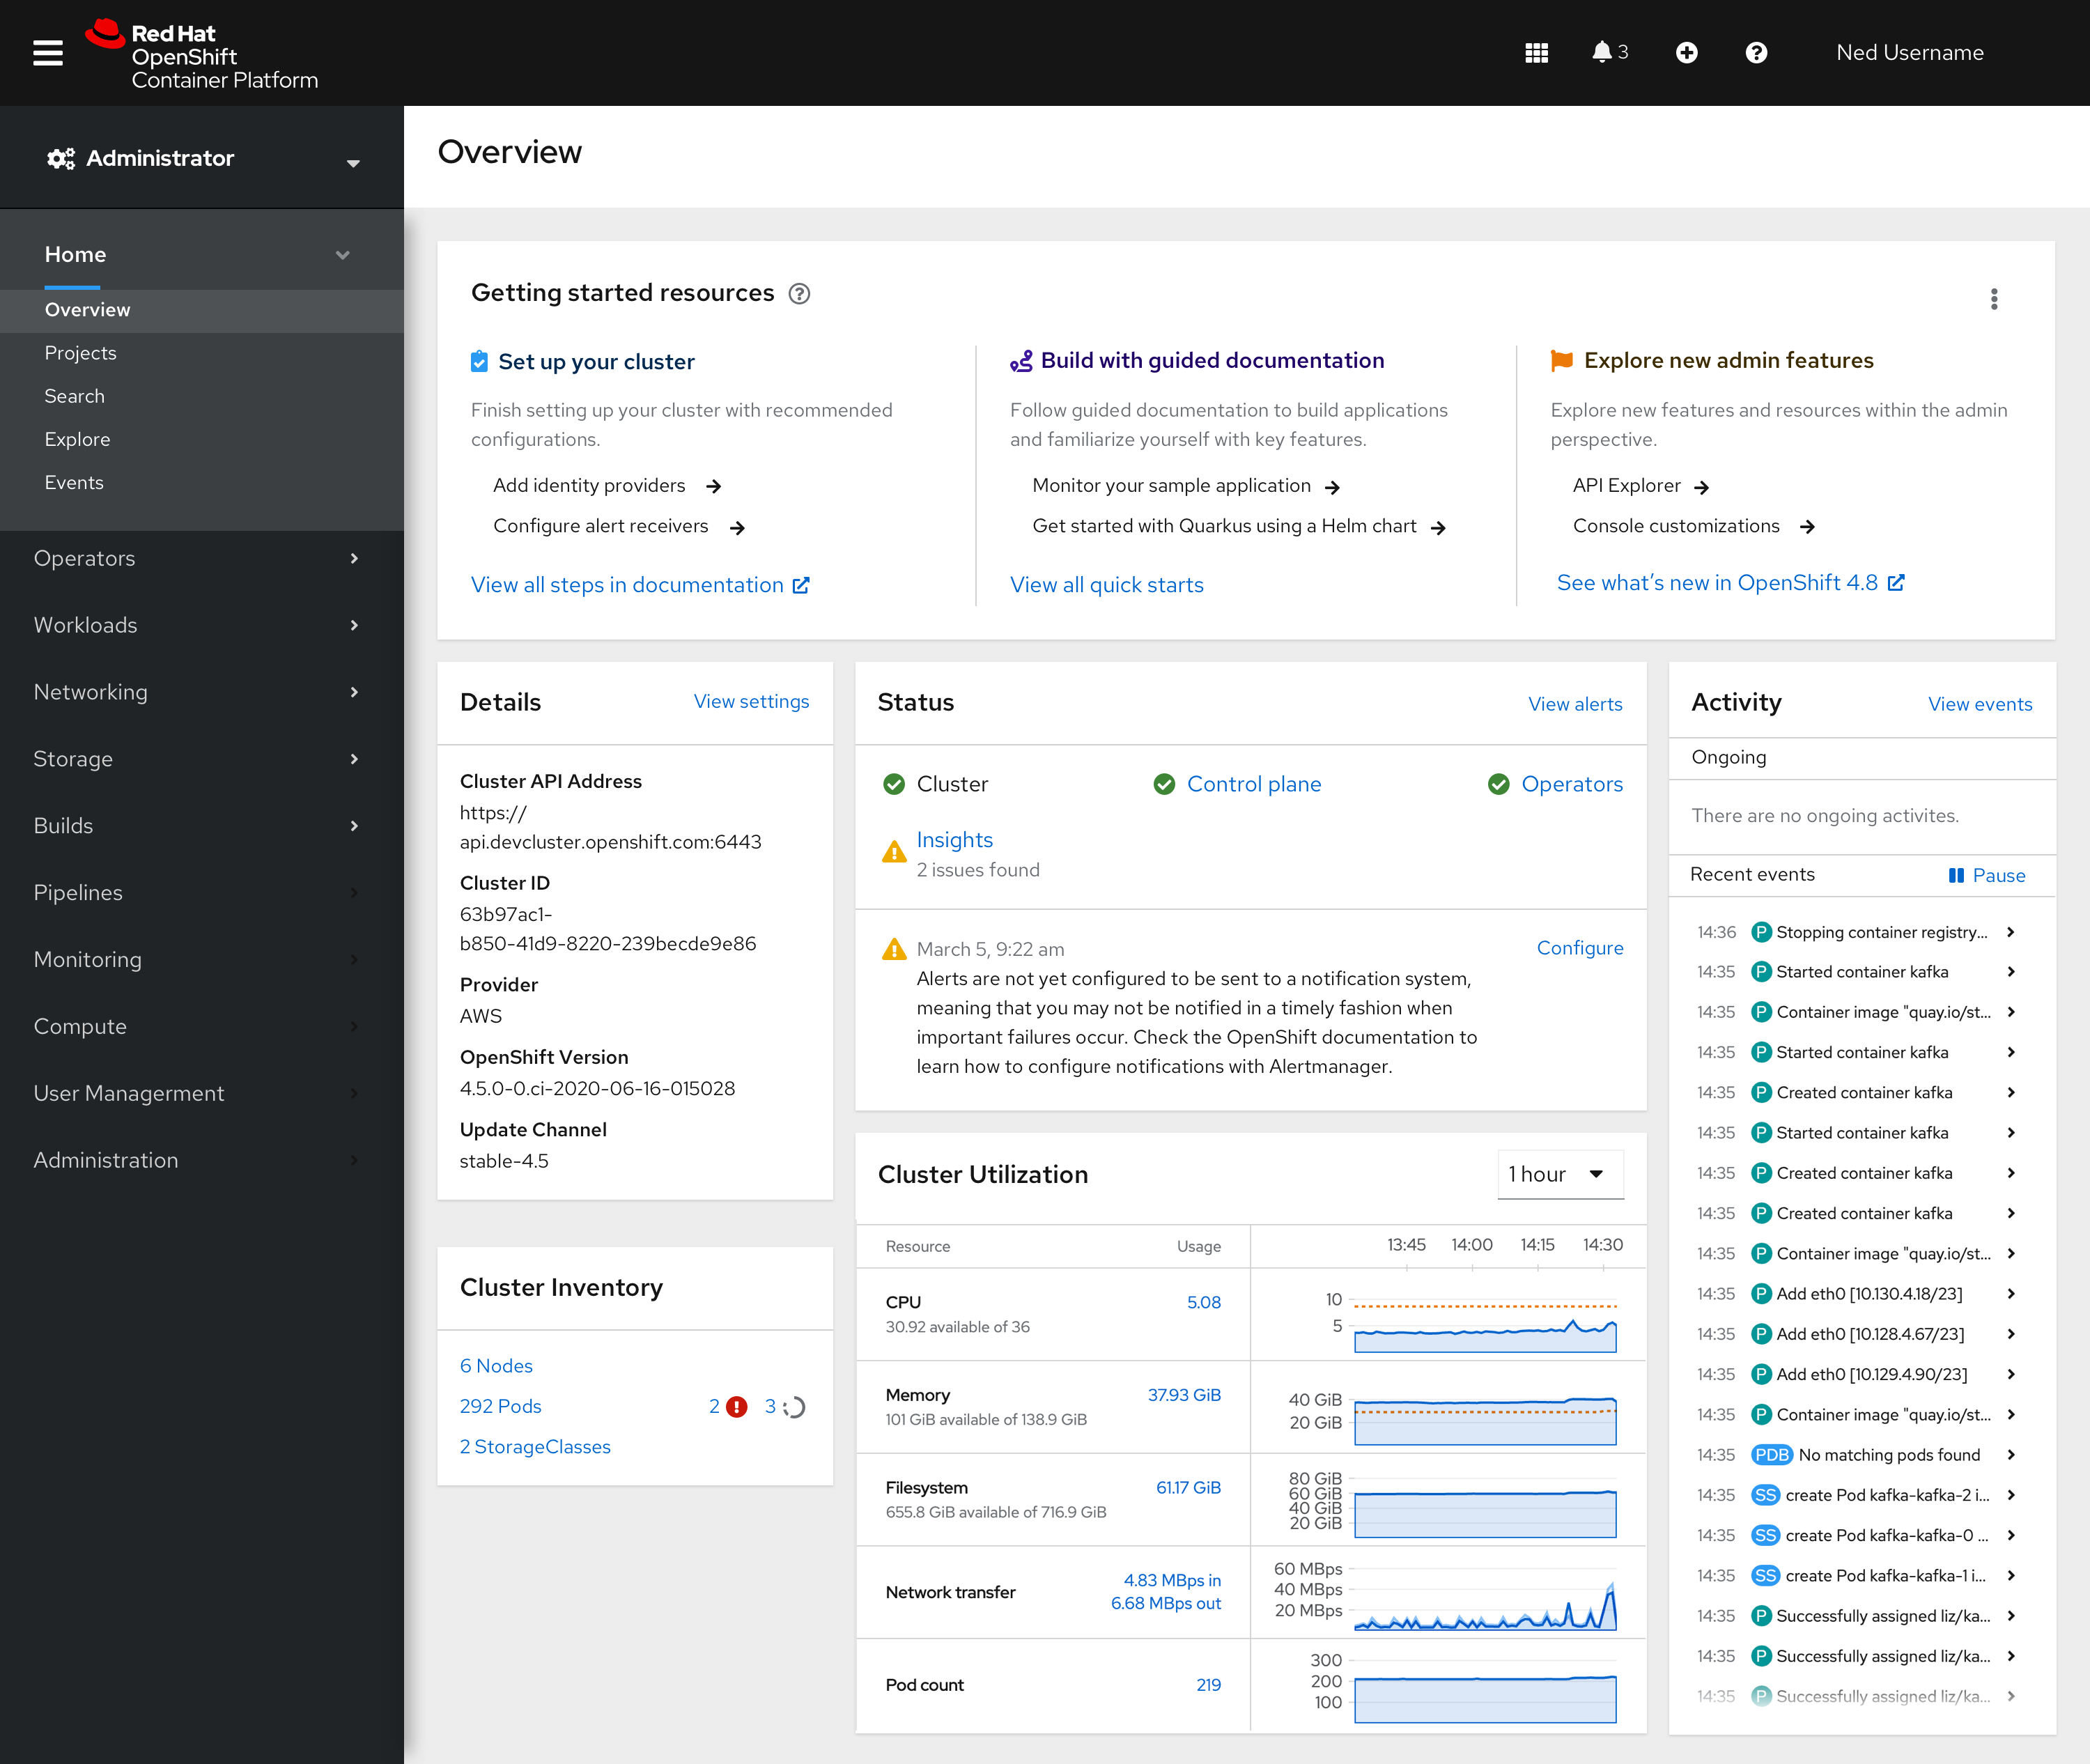
\includegraphics[width=0.85\textwidth]{images/openshift-dashboard.png}
        \caption{Openshift dashboard. Overview page.}
		\label{img:openshift-dashboard}
	\end{center}
\end{figure}

\subsubsection*{Rancher Desktop}

Rancher Desktop is ``an open-source application that provides all the essentials to work with containers and Kubernetes on the desktop'' \cite{rancher-desktop}.

Basically, it provides a local Kubernetes cluster with convenient GUI and a dashboard by default. It is widely used by developers to test their application in cloud environments without commiting the changes. 

Big advantage of Rancher Desktop is its simple installation process. Rancher Desktop is available for Windows, Linux and MacOS and is also bundled with all the necessary CLI tools like docker, nerdctl, kubectl, helm, and others.

Rancher Desktop allows to choose from dockerd or containerd as a container backend. Additionally, users can switch between Kubernetes versions easily to ensure compatibility with various environments. GUI allows to inspect containers and images, troubleshoot the cluster and forward container ports to the local machine. Figure~\ref{img:rancher-desktop} captures a ``Port Forwarding'' page of Rancher Desktop app.

Being free and easy to setup, Rancher Desktop became our main tool for local experiments. Most of our research was done on a Rancher local cluster. 

\begin{figure}[!hbt]
	\begin{center}
		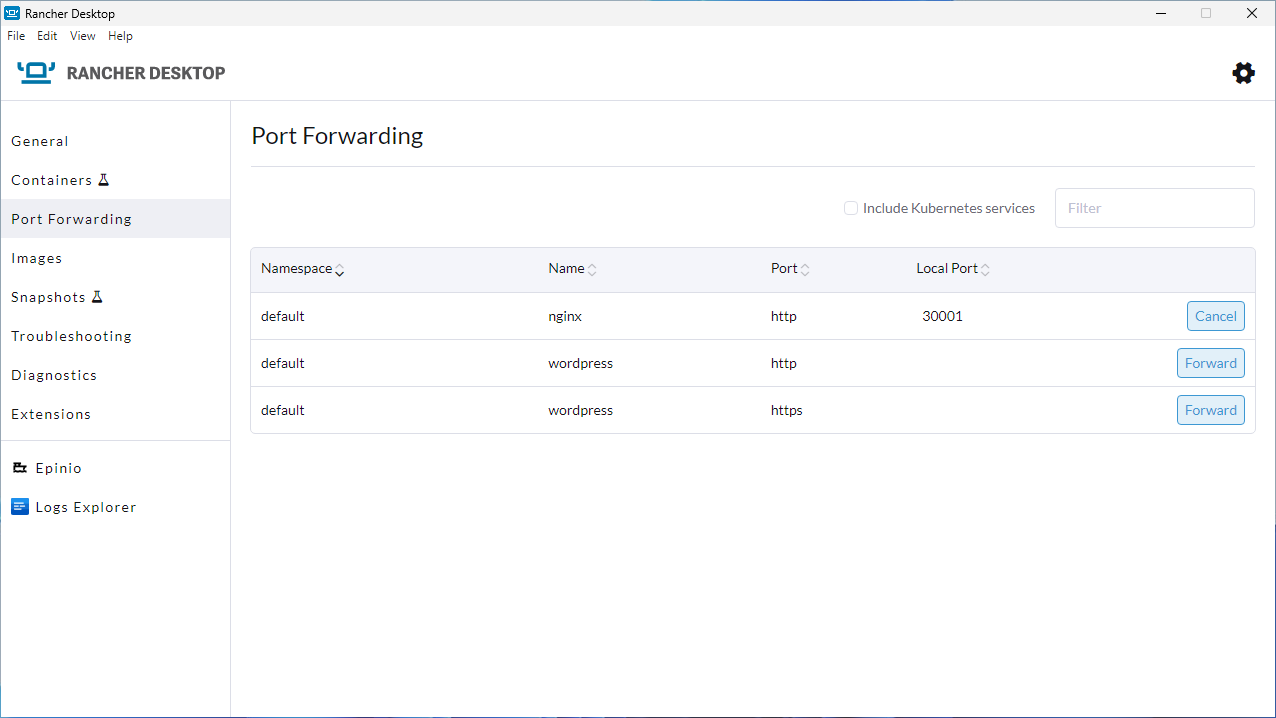
\includegraphics[width=0.85\textwidth]{images/rancher-desktop.png}
        \caption{Rancher Desktop GUI.}
		\label{img:rancher-desktop}
	\end{center}
\end{figure}